%!TEX root = ../VorlageBA.tex
\chapter{Grundlagen}

\section{Digital Imagery}
Digital imagery refers to visual content in digital form, that can be recognized and displayed by computers. For the purposes of this paper, we need to make a distinction between the following image types.

\begin{itemize}
	\item{Visible Spectrum(RGB) Imagery}
	\item{Thermal(Infrared) Imagery}
\end{itemize}

\subsection{Visible Spectrum(RGB) Imagery}

\cite{nasa_visiblelight} defines the visible light spectrum as the part of the electromagnetic spectrum visible to the human eye, ranging from approximately 380 to 700 nanometers in wavelength. This range encompasses all the colors perceivable by the human eye, from violet to red.

\subsection{Thermal(Infrared, IR) Imagery}
\cite{spi_thermal} defines thermal imaging, or thermography as the detection and measuring of radiation in the infrared spectrum being emitted from an object with the use of thermographic cameras. This type of imagery can collect temperature data from its field of view and display it using a variety of color palettes. Each pixel in a thermal image represents a temperature data point, and these data points are assigned a unique color or shade based on their value, meaning that as the thermal sensor detects changes in heat energy, it will express this change by adjusting the color or shade of a pixel. \citep{flir_colorpalette}

\begin{figure}[!ht]
	\centering
		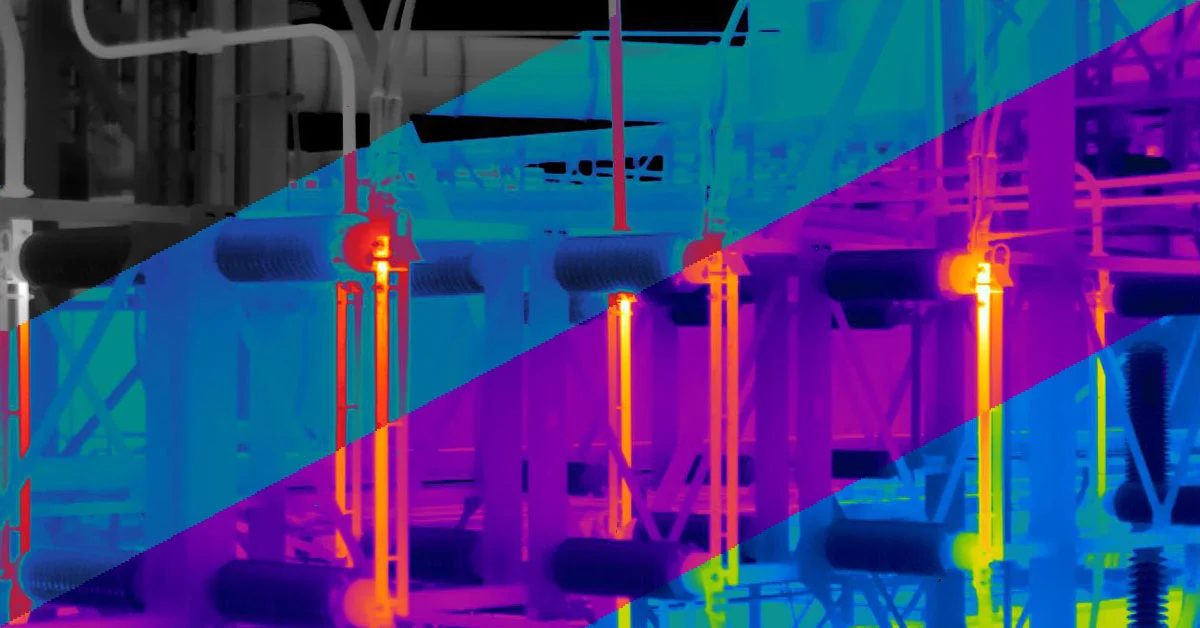
\includegraphics[width=0.75\textwidth]{images/color-palette-1200x628-fixed.png}
	\caption{Thermal Color Palettes \citep{flir_colorpalette}}
	\label{fig:color-palette}
\end{figure}

\section{Machine Learning (ML)}
\begin{quotation}
	\emph{``The studies reported here have been concerned with the
			programming of a digital computer to behave in a way
			which, if done by human beings or animals, would be
			described as involving the process of learning.''}
	\citep{samuel_machinelearning}
\end{quotation} 

Machine Learning is recognized to be a term originally coined by Arthur L. Samuel in \cite{samuel_machinelearning}. It refers to the behavior of a computer to learn by trial and error, improving it's performance on certain tasks by repeating those tasks over time. This essentially is how the computer trains for that task.

For a task to be fit for a machine learning application, a definite goal must exist, and at least one criterion or intermediate goal must exist which has a bearing on the achievement of the final goal and for which the sign should be known. \citep{samuel_machinelearning} Today, machine learning systems are used to identify objects in images, transcribe speech into text, match news items, posts or products with users’ interests, and select relevant results of search. \citep{deeplearning}

%TODO features and weights 

\begin{description}
\item[Supervised Learning] is a very common method of machine learning, where the training data contains the expected output of an ML model. The training algorithm can then compute an objective function that measures the error (or distance) between the output scores and the desired pattern of scores \citep{deeplearning} and adjust the feature weights to improve the result by minimizing the error.

\item[Unsupervised Learning], in contrast, does not contain any specific expected output within the training data. Thus the aim of the training is to recognize patterns within the dataset and categorize the data, rather than outputting a value that matches the correct and expected value.
\end{description}

\subsection{Deep Learning}
%TODO deep learning

	%TODO ML/DL optimizations

%TODO object detection

%TODO Object detection optimizations, feature selection, common algorithms and models etc.


%TODO örnek tezleri incele benzer grundlagen çıkar


